\section{System and Data}
\label{sec:system-data}

In this section, we describe our system implementation -- Android platform and Pebble platform, followed by a briefly cover of our the experiement setup.

\subsection{Android Platform}
\label{sec:android-platform}

Our Android application is adapted from BearLoc\footnote{BearLoc is developed by Software Defined Buildings (SDB) group at Berkeley; the intial goal of that project is to provide an open-source implementation for indoor semantic localization service.}. We built a continous sensor monitoring application on top of \texttt{BearLocService} which makes sensor data collection

Our initial application involves sampling all sorts of sensor data from Android platform, including acclerometer, gyroscope, magnetic field, light, GPS, WiFi signals, etc. However, through some preliminary study, we have found that mobile phones and Google Glass cannot easily handle the extensive sensing tasks, especially when we are trying to sample acceleration in a relative high frequency. As has discussed in Section~\ref{subsec: data-model}, since we are interested in the comparison among these wearable devices and Pebble only has a 3D accelerometer, we then restricted our Android application only for sampling acclerometer data.

The sensor data is obtained through \texttt{onSensorChanged()} API provided by Android OS. The sampling frequency is resource adaptive -- it turns out to be 100Hz for phones and 50Hz for Glass. 

Once the data is measured, we record the time in millisecond accuracy by calling \texttt{System.currentTimeMillis()}. To extract the data, we logged the data locally by writing to a \texttt{csv} file and also post a HTTP request that saves the data to \texttt{MongoDB}.

\subsection{Pebble Platform}
\label{sec:pebble-platform}

The Pebble accelerometer data collection application is based on \texttt{AccelerometerService} API provided by Pebble OS. We register a callback function as the handler whenever accelerometer data is available. The callback function operates on \texttt{AccelData} which already has a field of timestamp in millisecond accuracy. 

The data storage and transmission is supported by \texttt{DataLogging} API which requires a customized Android application that uses Pebble SDK to retrieve logs by application universally unique identifier (UUID). We have also developed this accompany Android application for retrieving the data and writing them into a \texttt{csv} file for data analysis.

\subsection{Accelerometer Data}
\label{sec:accelerometer-axes}

On both Android and Pebble platform, the acclerometer coordinate system is defined relative to the device's screen (see Figure~\ref{fig:coordinate}). When the user is facing the screen, the axes are:
\begin{itemize}
\item x: horizontal and points to the right.
\item y: vertical and points up.
\item z: points towards the outside of of the screen face.
\end{itemize}

 
%% 04-20 17:40:46.392    4187-4187/name.benzhang.hellostep.app I/HelloStep﹕ {Sensor name="MPL Accelerometer", vendor="Invensense", version=1, type=1, maxRange=19.6133, resolution=0.039226603, power=0.0, minDelay=1000}

%% { "_id" : ObjectId("536f303fe0323929bee2cf88"), "vendor" : "STMicroelectronics", "power" : 0.23000000417232513, "min delay" : 20000, "resolution" : 0.01362034771591425, "sysnano" : NumberLong("170075408653778"), "epoch" : NumberLong("1399795756898"), "version" : 1, "max range" : 19.613300323486328, "type" : "sensor info", "model" : "KR3DM 3-axis Accelerometer", "sensor" : "accelerometer", "id" : "9026086e-bd07-3f96-9622-757da2907a93" }

However, the data differs in range, resolution and sample frequency. We use $g$ to denote the gravitational accelerometer constant (normal $9.81 m/s^2$). In Table~\ref{tab:sensorinfo}, we have listed the sensor information. Note that these values are extracted from our hardware sensor API so they are device dependent. Our window frame based feature extraction (see Section~\ref{subsec: data-transform}) is immune to the discrepancy of sampling frequency.

\begin{table}
  \centering
  \begin{tabular}{c|c|c|c}
    \hline
    Device & max range & resolution & sample frequency \\
    \hline
    Phone  & 19.6g     & 0.013g     & 100Hz  \\
    Glass  & 19.6g     & 0.039g     & 50Hz   \\
    Pebble & 4g        & 0.008g     & 25Hz   \\
    \hline
  \end{tabular}
  \caption{Sensor information of the devices.}
  \label{tab:sensorinfo}
\end{table}

\begin{figure}
  \centering
  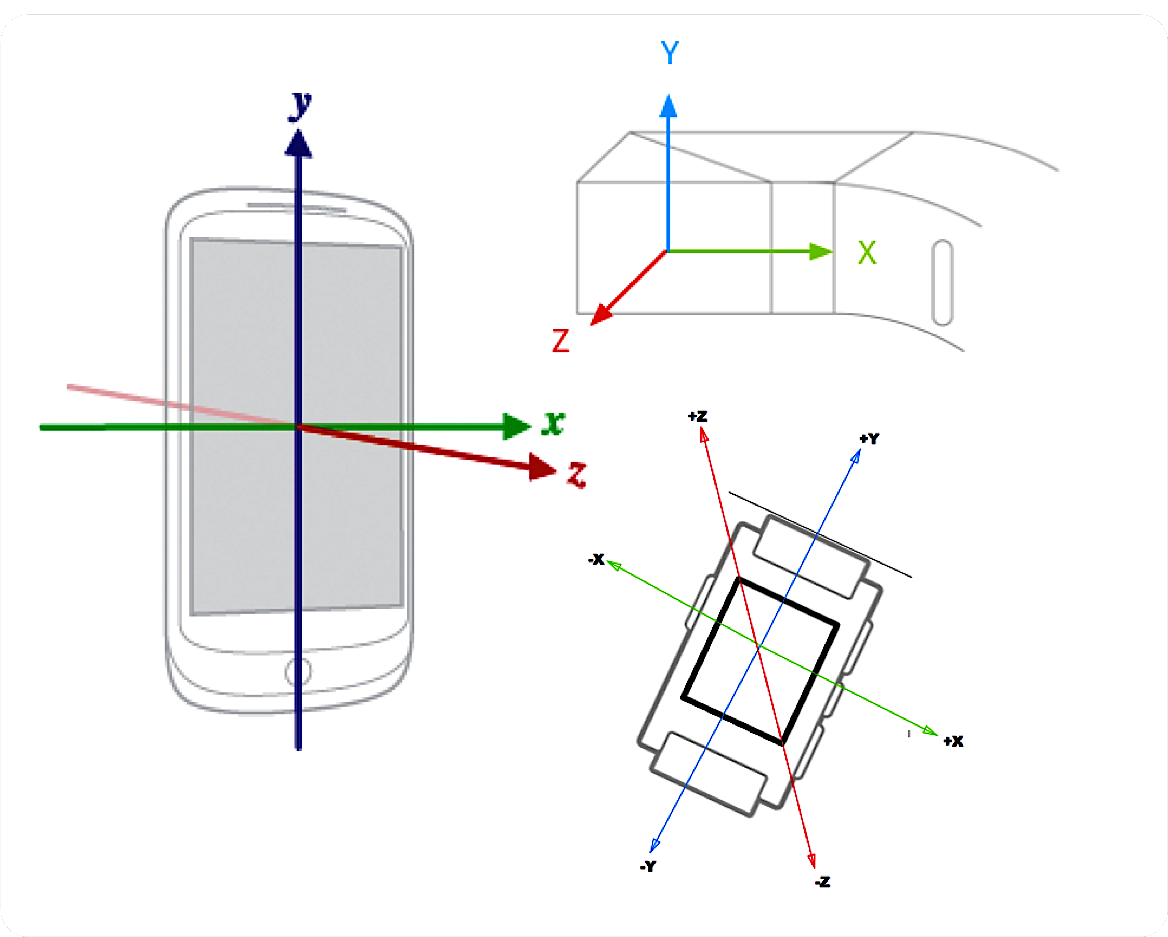
\includegraphics[width=0.9\columnwidth]{figures/coordinates.png}
  \caption{3D co-ordinate system of our hardware platforms.}
  \label{fig:coordinate}
\end{figure}

\vfill
\subsection{Data Collection}
\label{sec:data-collection-2}

With our data collection platform, we have performed a series of activities and collected the acclerometer data. Note that institutional review board (IRB) is a necessity for this kind of experiment if more volunteers are involved, thus for now the experiment is conducted by the authors. Figure~\ref{fig:exp} shows how these devices are worn on the author and the experiement is being conducted. To obtain the ground truth, we use an iPhone 5 to take videos continuously during the study. The video is manually processed to label the collected acclerometer data.

Two traces that we are using for this report were collected on May 10th. The author first walks out of a conference room, and then walk upstairs to 7th floor. He then pauses a while (standing) and then walk downstairs. After comning back to 4th floor, he passed the hallway by running. In such way we are able to collect all possible activities in one run. Notice that each activity duration is relatively random (some are quite short) which can be a challenge for a precise inference; however such randomness makes the data more realistic to people's normal life. 

\begin{figure}
  \centering
  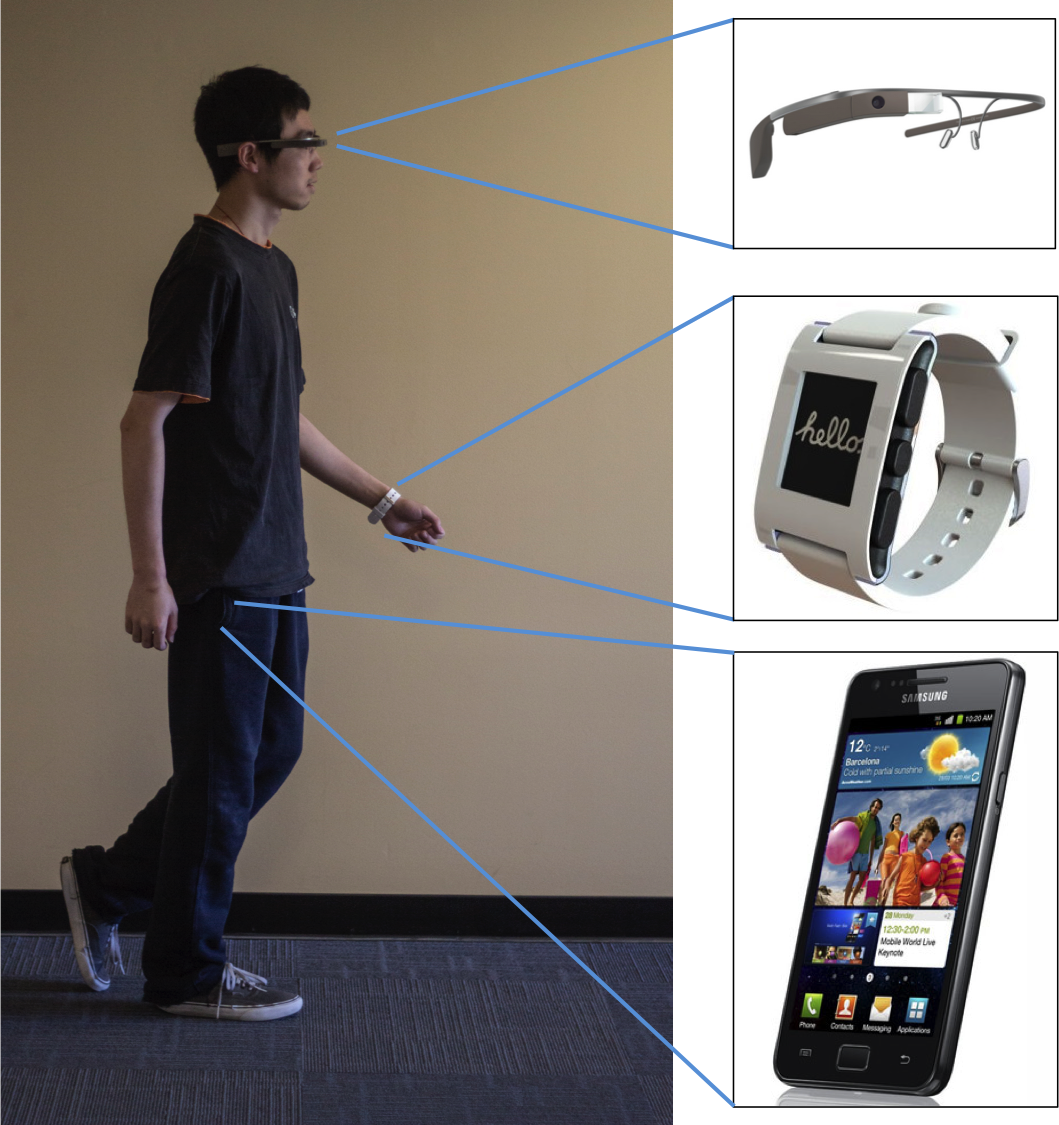
\includegraphics[width=0.9\columnwidth]{figures/experiement_setup.png}
  \caption{Data collection process of simutaneously wearing three different devices and an illustration of their relative positions on the author's body.}
  \label{fig:exp}
\end{figure}



%%% Local Variables: 
%%% mode: latex
%%% TeX-master: "main"
%%% End: 
